% Data flow diagram
% Author: David Fokkema
\documentclass{standalone}
\usepackage{xcolor}
\usepackage[tone]{tipa}
\let\ipa\textipa
\usepackage{tikz}
\usetikzlibrary{arrows,fit,calc,decorations.markings,positioning}
\tikzstyle{container} = [draw, very thick, dashed, rectangle, rounded
corners, inner sep=2.5em, fill = yellow!20 ]

\begin{document}

% Define the layers to draw the diagram
\pgfdeclarelayer{background}
\pgfdeclarelayer{foreground}
\pgfsetlayers{background,main,foreground}

%\begin{center}
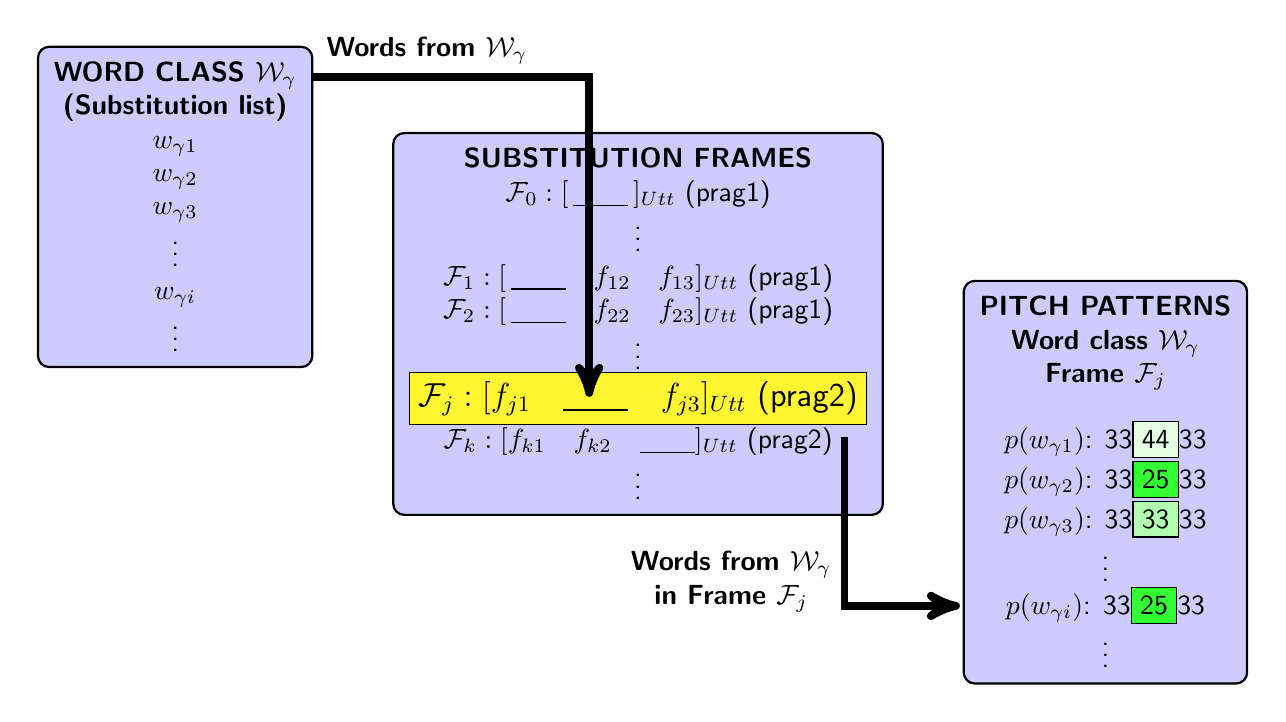
\begin{tikzpicture}[
  font=\sffamily,
  every matrix/.style={ampersand replacement=\&,column sep=1cm,row sep=-3cm},
  basic/.style={draw,thick,rounded corners,fill=blue!20,inner
    sep=.2cm, font=\sffamily\normalsize},
  sink/.style={basic,fill=green!20},
  dots/.style={gray,scale=2},
  to/.style={->,>=stealth',shorten >=1pt,thick,font=\sffamily\normalsize},
  every node/.style={align=center},
    decoration={
      markings,
      mark=at position 1 with {\arrow[scale=1,black]{triangle 60}};
    }
]


  % Position the nodes using a matrix layout
  \matrix{
    % Row 1
      \node[basic] (word) {\textbf{WORD CLASS $\mathcal{W}_{\gamma}$} \\
          \textbf{(Substitution list) } \\ $w_{\gamma 1}$ \\ $w_{\gamma 2}$ \\ $w_{\gamma 3}$
      \\ $\vdots$ \\ $w_{\gamma i}$ \\ $\vdots$};  \& \& \\
    % Row 2
      \& \node[basic] (sub) {\textbf{SUBSTITUTION FRAMES} \\
        $\mathcal{F}_0: [\,\underline{\qquad}\,]_{Utt}$ (prag1) \\
        $\vdots$ \\
      $\mathcal{F}_1: [\,\underline{\qquad}\quad f_{12} \quad
      f_{13}]_{Utt}$ (prag1)\\
      $\mathcal{F}_2: [\,\underline{\qquad}\quad f_{22} \quad
      f_{23}]_{Utt}$ (prag1)\\
      $\vdots$ \\
      \fcolorbox{black}{yellow!80}{\large{$\mathcal{F}_j:[f_{j1} \quad
          \underline{\qquad} \quad f_{j3} ]_{Utt}$} (prag2)}\\
      $\mathcal{F}_k: [f_{k1} \quad f_{k2}
      \quad\underline{\qquad} ]_{Utt}$ (prag2)\\
      $\vdots$}; \& \\
    % Row 3
       \& \&  \node[basic] (tone) {\textbf{PITCH
           PATTERNS}\\\textbf{Word class $\mathcal{W}_{\gamma}$}\\ \textbf{Frame $\mathcal{F}_j$}\\\\
         $p(w_{\gamma 1})$: \ipa{\tone{33}}\fcolorbox{black}{green!10}{\ipa{\tone{44}}}\ipa{\tone{33}} \\
         $p(w_{\gamma 2})$: \ipa{\tone{33}}\fcolorbox{black}{green!80}{\ipa{\tone{25}}}\ipa{\tone{33}} \\
         $p(w_{\gamma 3})$: \ipa{\tone{33}}\fcolorbox{black}{green!30}{\ipa{\tone{33}}}\ipa{\tone{33}} \\
         $\vdots$ \\
         $p(w_{\gamma i})$: \ipa{\tone{33}}\fcolorbox{black}{green!80}{\ipa{\tone{25}}}\ipa{\tone{33}} \\
      $\vdots$}; \\
%      \&\&\\ % Buffer row
      % Row 4
%    \node[sink] (classes) {\textbf{WORD CLASSES} \\ \textbf{(Substitution lists)}}; \& \& \\
    };


  \path[draw,to, line width = 1mm] ($(word.north east)+(0,-0.4)$)  -|
  node[above right,pos=0] {\textbf{Words from $\mathcal{W}_{\gamma}$}} ($(sub.north) + (-0.62,-3.4)$);

  \path[draw,to, line width = 1mm] ($(sub.south east)+(-0.5,1)$)  |-
  node[below left,pos=0.3] {\textbf{Words from
      $\mathcal{W}_{\gamma}$}\\\textbf{in Frame $\mathcal{F}_j$}} ($(tone.south west) + (0,1)$);


 % \node[container, fit=(phon) (morph)] (class) {};
 %    \node at (class.north) [above, node distance=0 and 0]
 %    {\textbf{Classify words by} \\ \textbf{morpho-phonological structure}};

 % \node[container, fit=(sub-frame) (tone)] (sub) {};
 %    \node at (sub.north) [above, node distance=0 and 0]
 %    {\textbf{Classify substitution items by pitch} \\ \textbf{in controlled contexts}};

 %    \node at (sub.north west) [below right, node distance=0 and 0]
 %    {\textbf{for OUT OF BLUE pragmatic context:}};

\end{tikzpicture}

\end{document}

    % Relative node placement
    \node[sink] at ($(class.west)-(1,0)$) [above] (unclassed)
    {\textbf{UNCLASSIFIED} \\ \textbf{WORDS}}; 

    \node[sink] at ($(class.east)+(1,0)$) [above] (classed) 
    {\textbf{WORD CLASSES} \\ \textbf{(Substitution lists)}}; 

    \node[sink] at ($(sub.east)+(1,0)$) [above] (tone-class) 
    {\textbf{TONE CLASSES} \\ \textbf{(Tentative)}}; 

  % Draw the arrows between the nodes and label them.
    \begin{pgfonlayer}{background}


  \path[draw,to, line width = 1mm] ($(unclassed.north)$)  |- node[above,pos=0] {} ($(morph.west)-(1,0)$);

  \path[draw,to, line width = 1mm] ($(phon.east)+(1,0)$)  -| node[above,pos=0] {} ($(classed.south)-(0.3,0)$);

  \path[draw,to, line width = 1mm] ($(tone.east)+(1,0)$)  -| node[above,pos=0] {} ($(tone-class.south)+(0.3,0)$);


    \path[draw,to, line width = 1mm] ($(classed.north)+(0.3,0)$)  |-
    node[above right=0.4mm of classed] {Class 1} ($(sub-frame) -(3.5,0)$);

  \path[draw,to, line width = 1mm] ($(classed.north)+(0.3, 0)$) |-
  node[above right=0.4mm of classed] {Class 2} ($(sub-frame) -(3.5,0.5)$);

  \path[draw,to, line width = 1mm] ($(classed.north)+(0.3, 0)$) |-
  node[above right=0.4mm of classed] {Class 3} ($(sub-frame) -(3.5,1)$);

  \path[draw,to, line width = 1mm] ($(classed.north)+(0.3, 0)$) |-
  node[above right=0.4mm of classed] {Class 4} ($(sub-frame) -(3.5,1.5)$);

  \path[draw,to, line width = 1mm] ($(classed.north)+(0.3, 0)$) |-
  node[above right=0.4mm of classed] {Class 5} ($(sub-frame) -(3.5,2)$);

  \path[draw,to, line width = 1mm] ($(classed.north)+(0.3, 0)$) |-
  node[above right=0.4mm of classed] {Class 6} ($(sub-frame) -(3.5,2.5)$);

  \path[draw,to, line width = 1mm] ($(classed.north)+(0.3, 0)$) |-
  node[above right=1mm of classed] {$\vdots$} ($(sub-frame) -(3.5,3)$);

  \path[draw,to, line width = 1mm] ($(classed.north)+(0.3, 0)$) |-
  node[above right=0.4mm of classed] {Class $i$} ($(sub-frame) -(3.5,3.5)$);

  \path[draw,to, line width = 1mm] ($(classed.north)+(0.3, 0)$) |-
  node[above right=1mm of classed] {$\vdots$} ($(sub-frame) -(3.5,4)$);

  \path[draw,to, line width = 1mm] ($(classed.south)+(0.3,0)$)  |-
  node[above right=0.4mm of classed] {Class $n$} ($(tone) -(3.5,0)$);

  \path[draw,to, line width = 1mm] ($(classed.north)+(0.3, 0)$) |-  ($(sub-frame) -(3.5,0.5)$);

\draw[draw, to, line width = 1mm] ($(tone.south)+(-2,-1)$) to[bend right=60]
node[below=1mm of tone]  {\textbf{REPEAT FOR EACH} \\ \textbf{SUBSTITUTION FRAME}} ($(tone.south)+(2,-1)$);

\end{pgfonlayer}

\end{tikzpicture}
%\end{center}
\end{document}
